%% progress-report-8-SubmapVisualization+ROSPackage tex file.
%% Completed By Yuyang Rong(rongyy@shanghaitech.edu.cn) and
%% Jianxiong Cai(caijx@shanghaitech.edu.cn)
%%
%% To edit this file, please use indentions with tab size of 2.
%%

%% File name unchanged. This is just a temp file.

\documentclass[conference,compsoc]{IEEEtran}
\usepackage{cite}
\usepackage{listings}
\usepackage{blindtext}
\usepackage{enumitem}
% for coding highlight
\usepackage{graphicx}
\usepackage[colorlinks=true,urlcolor=blue]{hyperref}
\usepackage{amsmath, amsthm, amssymb}
\usepackage{subfloat}
\usepackage{ulem}
\usepackage{indentfirst}
\newcommand{\subparagraph}{}
\begin{document}
\title{
	Deep Learning Course Proposal \\
	Passenger Screening Algorithm Challenge \\
}


% author names and affiliations
% use a multiple column layout for up to three different
% affiliations
\author{
	\IEEEauthorblockN{Yuyang Rong}
	\IEEEauthorblockA{
		School of Information Science and Technology \\
		ShanghaiTech University \\
		Student ID: 69850764 \\
	}
\and
	\IEEEauthorblockN{Peng Ding}
	\IEEEauthorblockA{
		School of Information Science and Technology \\
		ShanghaiTech University \\
		Student ID: xxxxxxxx \\
	}
}

\maketitle

\begin{abstract}
	It has becoming more and more important to guarantee passenger's safety when they are traveling by air. One important thing to do is to check if any passenger is carrying dangerous things. Traditionally we take scans of passengers and let human decide, however, such approach is time waisting and inaccurate. We are going to use deep learning methods to decide that, among 17 critical positions of a human scan, whether he carries dangerous entities or not.
\end{abstract}
\section{Introduction}
	\par
	This is a challenge proposed in kaggle.com, asking for algorithms that can detect dangerous things based on scans in airport. Traditional human labor can be problematic and time consuming and most importantly, inaccurate. How can we apply learning knowledge to tackle such a problem has become not only interesting but also beneficial to all the passengers' personal safety.
	\par 
	In our work we will be focusing on 17 positions of a human body, listed below:
	\begin{figure}[h]
		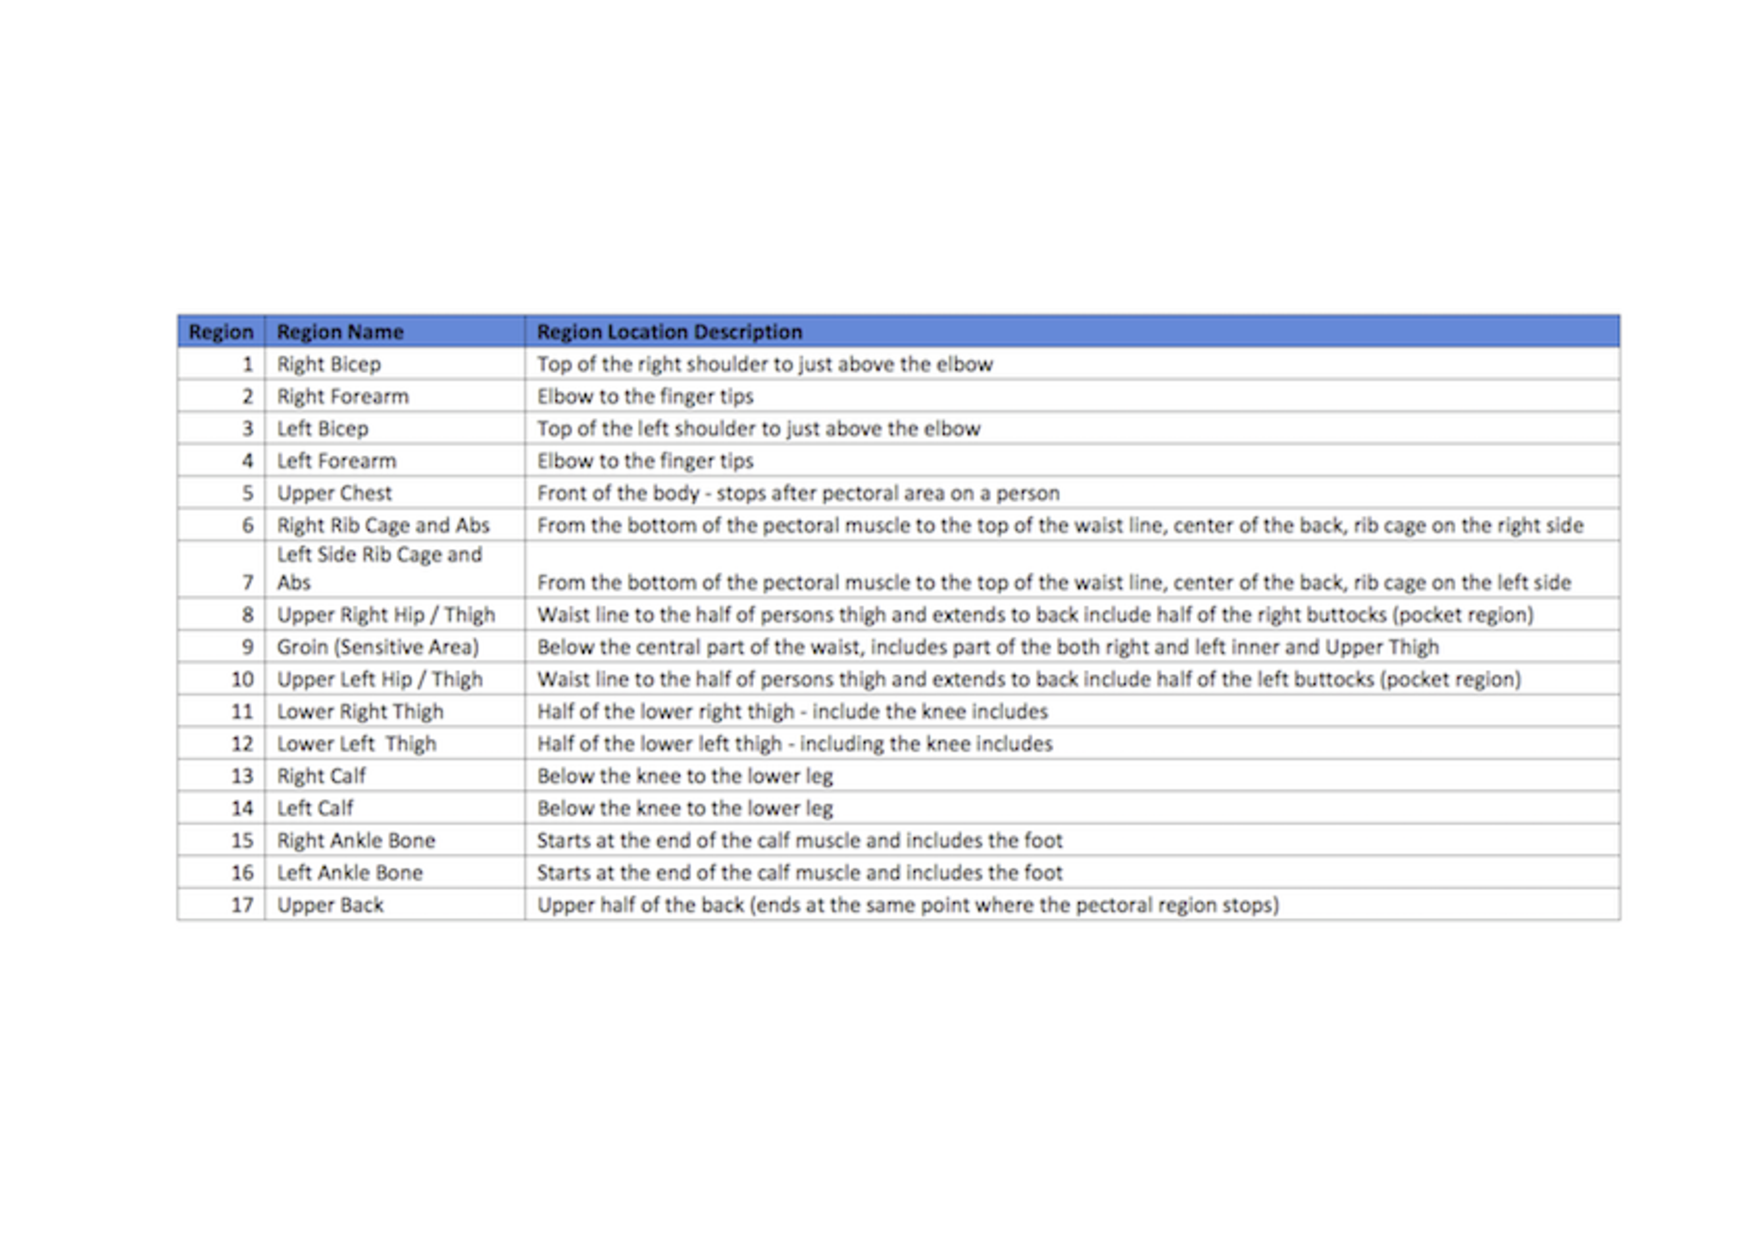
\includegraphics[scale=0.3]{Pic/body_zones.pdf}
		\caption{17 regions of a human body}
	\end{figure}
\section{Data}
	We will be using data provided by kaggle.com, to be more precise, by Department of Homeland Security. All the data are in the following four formats:
	\begin{itemize}
		\item{*.ahi} Calibrated object raw data file.
		\item{*.aps} Projected image angle sequence file.
		\item{*.a3d} Combined image 3D file.
		\item{*.a3daps} Combined image angle sequence file.
	\end{itemize}
\section{Related Work}
	As deep learning has been successful in object recognition. 
	TODO What?
\section{Approach}
	ConvNet
	TODO Be specific.
\section{Experiments}
	We will be doing experiments on validation set to tune our parameters. We will compare the loss function of the prediction and the ground truth. The loss function is defined as: \\
	If there are $N$ images, there will be $17N$,
	$$ L = -\frac{1}{N}\sum_{i=1}^N{y_i\log(\hat{y}_i) + (1-y_i)log(1-\hat{y}_i)}$$
	We may also be plotting the function of loss in terms of each parameters.
\section{Evaluation}
	The final evaluation will not be limited to validation set, but we will evaluate our system based on the rating algorithm proposed by kaggle.com. That will have to wait until we submit our work.



\bibliographystyle{IEEEtran}
%% De-comment this line if you have any reference.
%% And don't forget to change .bib file.
%\bibliography{proposal}
\end{document}
